\cleardoubleoddpage
\chapter{Materials}
\label{app:Datasets_and_the_Environment}

\section{The Lunar Lander Environment}
\label{sec:the_lunar_lande_environment}

All experiments in this work were conducted in the Lunar Lander v2 environment \cite{LunarLanderEnv}, a classical RL benchmark simulating a rocket trajectory optimization task. The agent’s objective is to land a spacecraft safely, preferably on a designated landing pad, while maintaining stability and minimizing fuel consumption.

The environment has a discrete action space and a continuous state space. The state is represented as an 8-dimensional vector: $x$ and $y$ coordinates, linear velocities along the $x$- and $y$-axes ($lv_x$ and $lv_y$), lander orientation angle, angular velocity, and binary indicators for left and right leg ground contact. The action space consists of four discrete actions: 0 - do nothing, 1 - fire the left orientation engine, 2 - fire the main engine, and 3 - fire the right orientation engine.

Environment dynamics are deterministic, meaning that selected actions are the ones being executed. However, a small stochastic component is introduced at episode initialization - small random forces are applied to the lander in the initial state, mainly affecting linear and angular velocities. This stochasticity can create out-of-distribution states, which is particularly relevant in the offline RL context due to the potential for extrapolation error \cite{lange2012batch}.

The reward structure is designed to encourage precise, stable, and fuel-efficient landings. Positive rewards are granted for being close to the landing pad, maintaining controlled descent, and keeping the lander upright, while penalties are applied for high velocities, unnecessary engine usage, or crashes. Additional components include $+10$ per landing leg contact, $-0.03$ per timestep for side engine use, $-0.3$ per timestep for main engine use, $+100$ for a successful landing, and $-100$ for crashing.

Therefore, from the given domain knowledge we can conclude that an optimal policy gradually lowers the lander while maintaining stability, minimizes side engine usage, and ensures that both landing legs make contact with the ground. This aligns with both domain knowledge and the environment’s reward signal definitions \cite{LunarLanderEnv}.




\section{Offline Datasets}
\label{sec:the_learning_pipeline}
To study the effect of data composition in the offline DQN+BC setting, two offline datasets are used: a Replay Buffer (RB) dataset and a Final Policy (FP) dataset. Both datasets consist of state-action pairs collected from an online DQN agent \cite{DQN} interacting with the Lunar Lander environment \cite{LunarLanderEnv}.


The datasets differ in how the experience was generated. The RB dataset contains transitions collected throughout online training, capturing multiple evolving, exploratory, and sub-optimal policies. In contrast, the FP dataset contains transitions collected after training was finished and represents a single, near-optimal, and consistent policy. This distinction allows for a systematic analysis of how data quality, composition, and diversity affects offline RL performance.




\subsection{Data splits}
For both the RB and FP datasets, the data is split into three subsets to support supervised learning and offline RL experiments: a training subset used for model training and data exploration, a validation subset for model evaluation, early stopping, and pruning techniques during hyperparameter tuning, and a test subset reserved for final evaluation after all training and tuning. The split ratio is $80\%$ training, $10\%$ validation, and $10\% $test.

To prevent data leakage, splitting is performed at the episode level: all state-action pairs from a given episode were assigned to exactly one subset. This ensures that transitions from the same episode do not appear across multiple subsets, maintaining a clean separation between training, validation, and testing data.

Furthermore, all statistical and coverage analysis, dataset exploration, normalization statistics, and feature importance calculations are performed exclusively on the training subsets. Validation and test subsets are not used for these purposes, guaranteeing that model evaluation reflects genuine generalization to unseen data.





\section{Dataset Statistics, Coverage and Exploration}

Data exploration was conducted based on the training subsets of the RB and FP datasets, using summary statistics and Kernel Density Estimation (KDE) plots to investigate the distributions of state and reward features. Mean and standard deviation (SD) values were computed for all continuous state dimensions as well as for the current immediate reward. The results are summarized in Table~\ref{tab:data_exploration_summary_statistics}.

\subsection{State Features}

To compare behaviour between the RB and FP datasets, we examined all continuous state dimensions using summary statistics and KDE plots. This analysis captures both the general tendencies and variability of the data, highlighting the consistency of FP behaviour vs the broader exploration in RB. KDE plots of the individual state features are shown in Figure~\ref{fig:rb_fp_univar}.


\begin{enumerate}[label=\textbullet]
    \item \textbf{X-coordinates (Horizontal position):} Both datasets are centered around zero (RB: $0.0030$, FP: $-0.0323$) with relatively small variance (RB SD: $0.3170$, FP SD: $0.2806$). KDE plots (Figure~\ref{fig:rb_fp_univar}) indicate substantial overlap, showing that trajectories in both datasets remain generally horizontally centered.

    \item \textbf{Y-coordinates (Vertical position):} The FP dataset shows lower mean values (FP: $0.4578$ vs RB: $0.6293$) and slightly lower SD (FP: $0.3664$, RB: $0.3922$). KDEs suggest FP trajectories are lower and concentrated closer to the ground, while RB trajectories cover a wider vertical range.

    \item \textbf{$lv_x$ (Linear velocity in $x$):} Mean values are near zero (RB: $-0.0047$, FP: $-0.0212$), with FP showing lower variance (SD FP: $0.2041$ vs SD RB: $0.2586$). KDE plots highlight tighter FP distributions with fewer extreme values.

    \item \textbf{$lv_y$ (Linear velocity in $y$):} Both datasets have negative means, suggesting downward motion (FP: $-0.0734$, RB: $-0.0854$). FP shows significantly lower SD ($0.0884$ vs $0.1874$), indicating slower and more consistent descent compared to RB trajectories.

    \item \textbf{Orientation angle:} Means are near zero (RB: $0.0031$, FP: $-0.0005$), with FP showing tighter distributions (SD FP: $0.0583$ vs SD RB: $0.1385$). KDE plots indicate more stable lander orientation in FP datapoints.

    \item \textbf{Angular velocity:} Both datasets have near-zero means, but FP shows significantly lower variance (SD FP: $0.0422$ vs SD RB: $0.0977$), suggesting smoother rotational behavior.
\end{enumerate}

\subsection{Reward}

The RB dataset has a negative mean reward ($-0.1799$), while the FP dataset has a positive mean ($0.0978$). Both datasets show relatively high SD (around 3.5). KDE plots of accumulated rewards (Figure~\ref{fig:rb_fp_reward_analysis}) reveal similar multimodal shapes, with FP distributions shifted toward higher current reward.

\begin{figure}[!b]
\centering
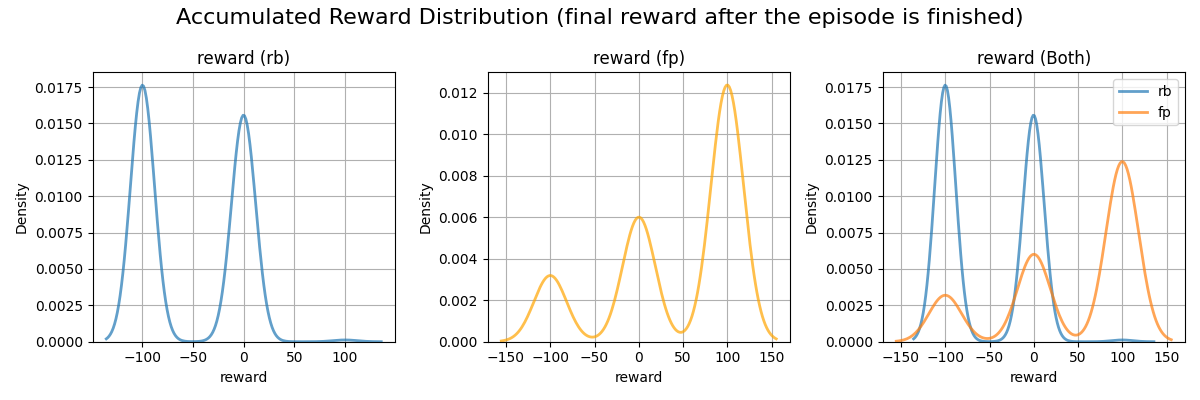
\includegraphics[width=1\linewidth]{images/data_exploration/rb_fp_reward_analysis_fig.png}
\caption{
KDE plots of the accumulated rewards of the original online DQN agent collected per episode for the RB and FP datasets.
}
\label{fig:rb_fp_reward_analysis}
\end{figure}

\begin{table}[!ht]
\centering
\caption{Mean and SD statistics for RB and FP training subsets}
\label{tab:data_exploration_summary_statistics}

\renewcommand{\arraystretch}{1.2}  % increase row height
\resizebox{\textwidth}{!}{%
\begin{tabular}{l c c c c c c c c}
\hline
\textbf{Dataset} 
& \textbf{Metric} 
& \textbf{$x$} 
& \textbf{$y$}
& \textbf{$lv_x$} 
& \textbf{$lv_y$} 
& \textbf{angle}
& \textbf{angular velocity}
& \textbf{reward} \\
\hline
\multirow{2}{*}{\textbf{RB}} & \textbf{Mean} & 0.0030 & 0.6293 & -0.0047 & -0.0854 & 0.0031 & 0.0005 & -0.1799 \\
                    & \textbf{SD} & 0.3170 & 0.3922 & 0.2586 & 0.1874 & 0.1385 & 0.0977 & 3.5129 \\
\multirow{2}{*}{\textbf{FP}} & \textbf{Mean} & -0.0323 & 0.4578 & -0.0212 & -0.0734 & -0.0005 & -0.0005 & 0.0978 \\
                    & \textbf{SD} & 0.2806 & 0.3664 & 0.2041 & 0.0884 & 0.0583 & 0.0422 & 3.4109 \\
\hline
\end{tabular}
}
\end{table}

\begin{figure}[!b]
\centering
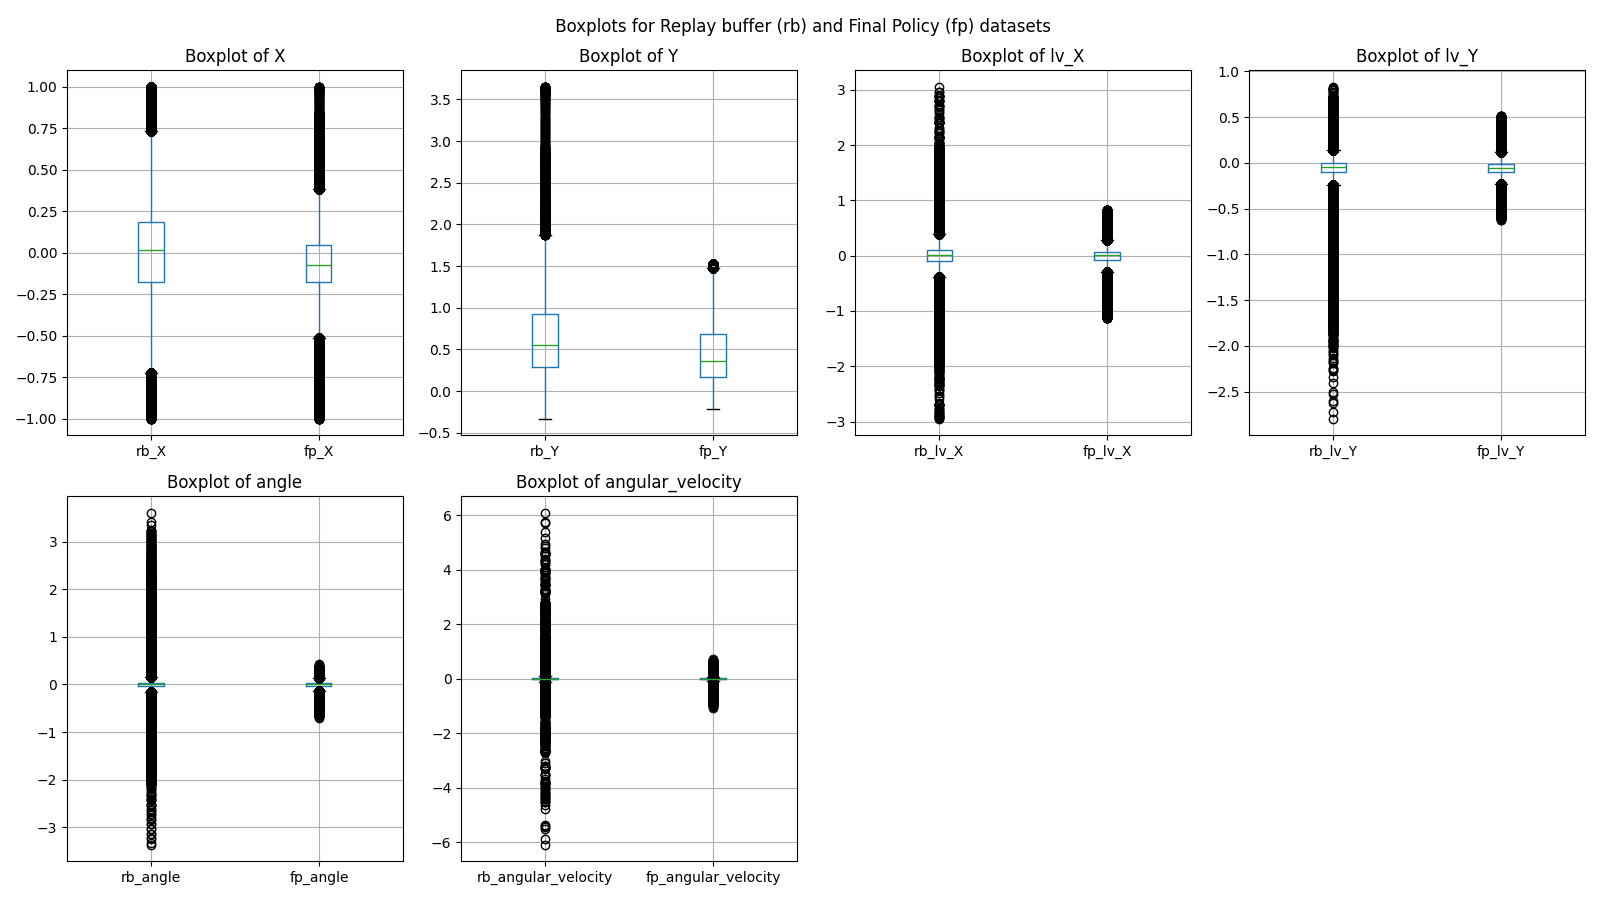
\includegraphics[width=1\linewidth]{images/data_exploration/rb_fp_boxplots_combined_fig.png}
\caption{
Boxplots constructed for all continuous features of the RB and FP training data subsets. All statistics are computed exclusively on the training data to avoid information leakage.
}
\label{fig:rb_fp_boxlots}
\end{figure}

\begin{figure}[!b]
\centering
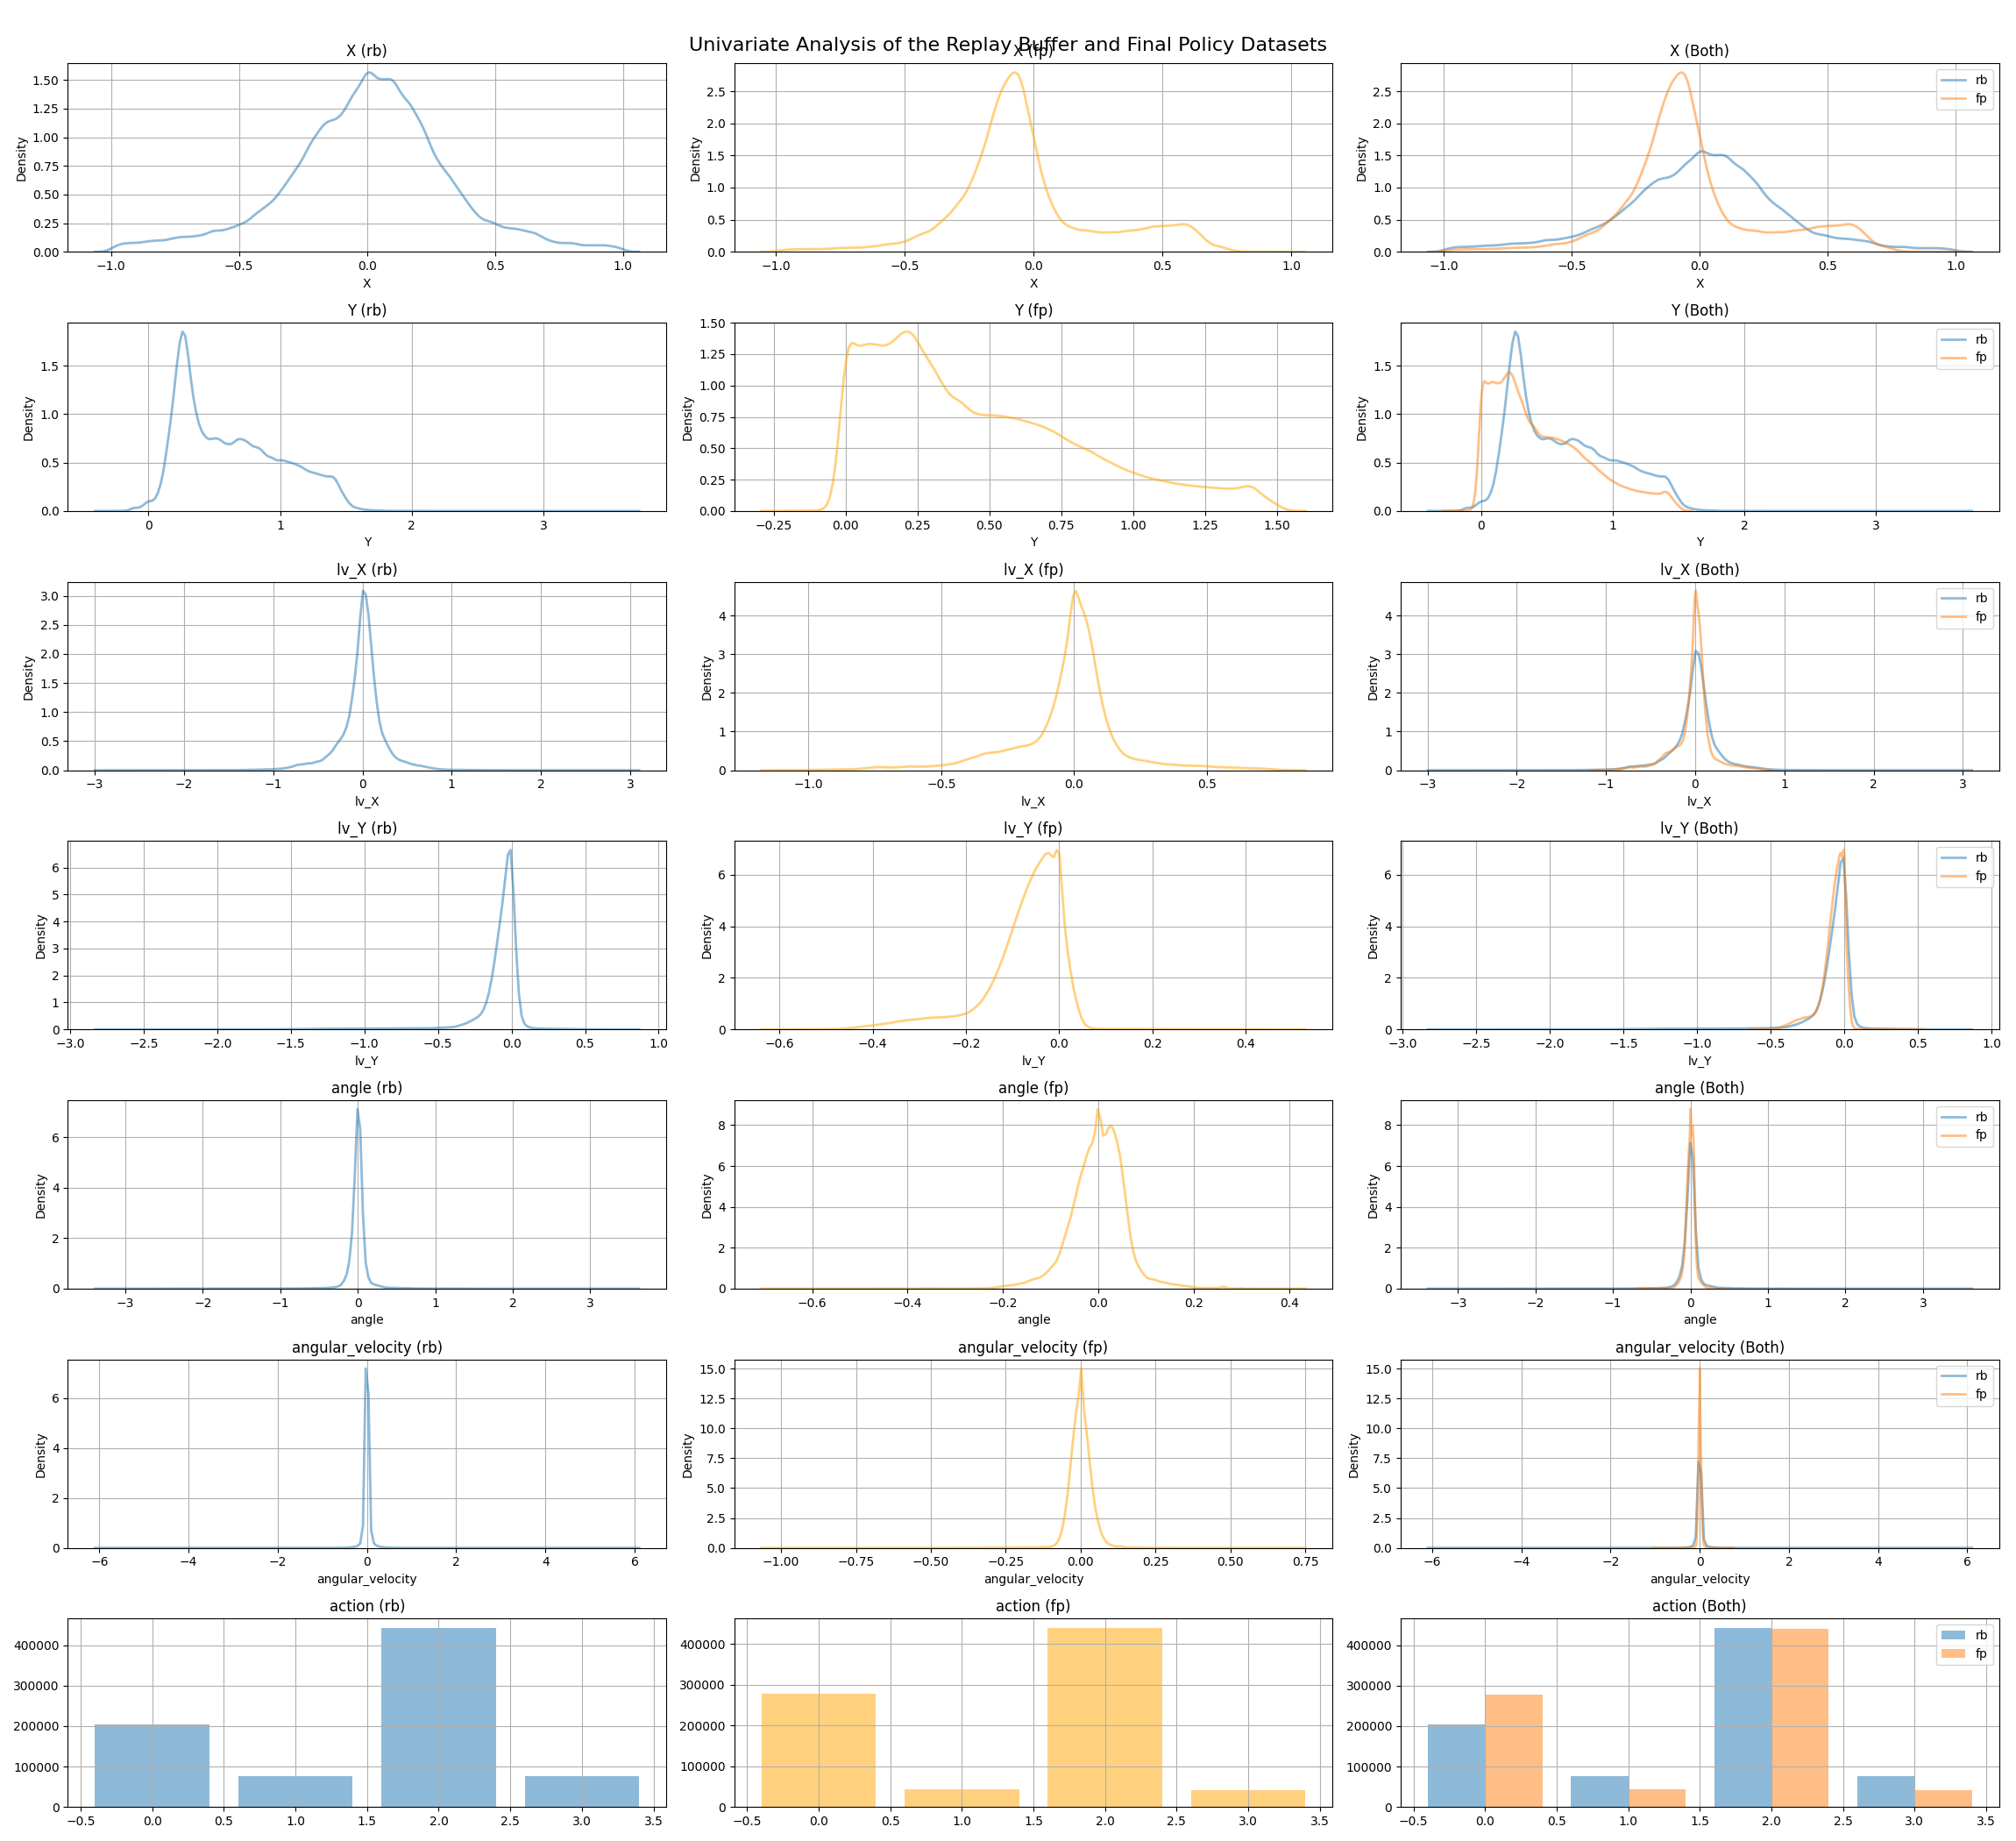
\includegraphics[width=1\linewidth]{images/data_exploration/rb_fp_univar_fig.png}
\caption{
KDE plots and histograms for some of the features across the training RB and FP data subsets. All statistics are computed exclusively on the training data to avoid information leakage. Overall, the RB dataset exhibits greater variability in state distributions, reflecting more exploratory behaviour, while the FP dataset shows more concentrated states, indicating consistent and stable policy execution.}
\label{fig:rb_fp_univar}
\end{figure}


\noindent\textbf{IMPORTANT NOTE:} The state features and rewards are not independent and identically distributed (I.I.D). Many are functionally related - for example, angular velocity depends on $lv_x$ and $lv_y$. This is reflected in the correlation matrices (Figure~\ref{fig:correlation_matrices}), showing that several features are strongly correlated. This observation should be taken into consideration later on when we discuss deep learning model architectures.










\section{State Normalization}
State normalization was applied as a preprocessing step to improve stability and support learning for both supervised BC models and offline DQN+BC agents. All normalization parameters, including but not limited to minimum, maximum, mean, standard deviation, and quintiles, were computed exclusively on the training subset of each dataset (RB or FP) to prevent data leakage. These parameters were then applied unchanged to the corresponding validation and test subsets, as well as to all models trained under the same configuration.

For each dataset, multiple normalized versions of the state space are created to evaluate the effect of different normalization strategies, while the raw, non-normalized state representation is kept as a baseline for comparison. The normalization techniques considered in this work include:

\begin{itemize}
    \item \textbf{Min-Max normalization [0,1]:} Scales each feature independently to the interval $[0,1]$, ensuring bounded inputs for NN training:
    
    $$x_\text{norm} = \frac{x - x_\text{min}}{x_\text{max} - x_\text{min}}$$
    

    \item \textbf{Max-Abs normalization [-1,1]:} Scales each feature by its maximum absolute value, preserving exact zeros and negative signs in the state:
    
    $$x_\text{norm} = \frac{x}{|x_\text{max}|}$$
    

    \item \textbf{Standard (z-score) normalization:} Centers each feature around zero with unit variance ($\sigma = 1$). Follows the implementation used in TD3+BC \cite{fujimoto2021minimalist} where z-score state normalization is applied during training:

    $$x_\text{norm} = \frac{x - x_\text{mean}}{x_\text{std} + \epsilon}$$


    \item \textbf{Robust normalization:} Uses the median and inter-quartile range to reduce sensitivity to outliers, might be particularly useful for the RB dataset where there are many outliers:
    $$x_\text{norm} = \frac{x - x_\text{median}}{x_{Q3} - x_{Q1}}$$
\end{itemize}






\section{Feature Importance}

\begin{figure}[!b]
\centering
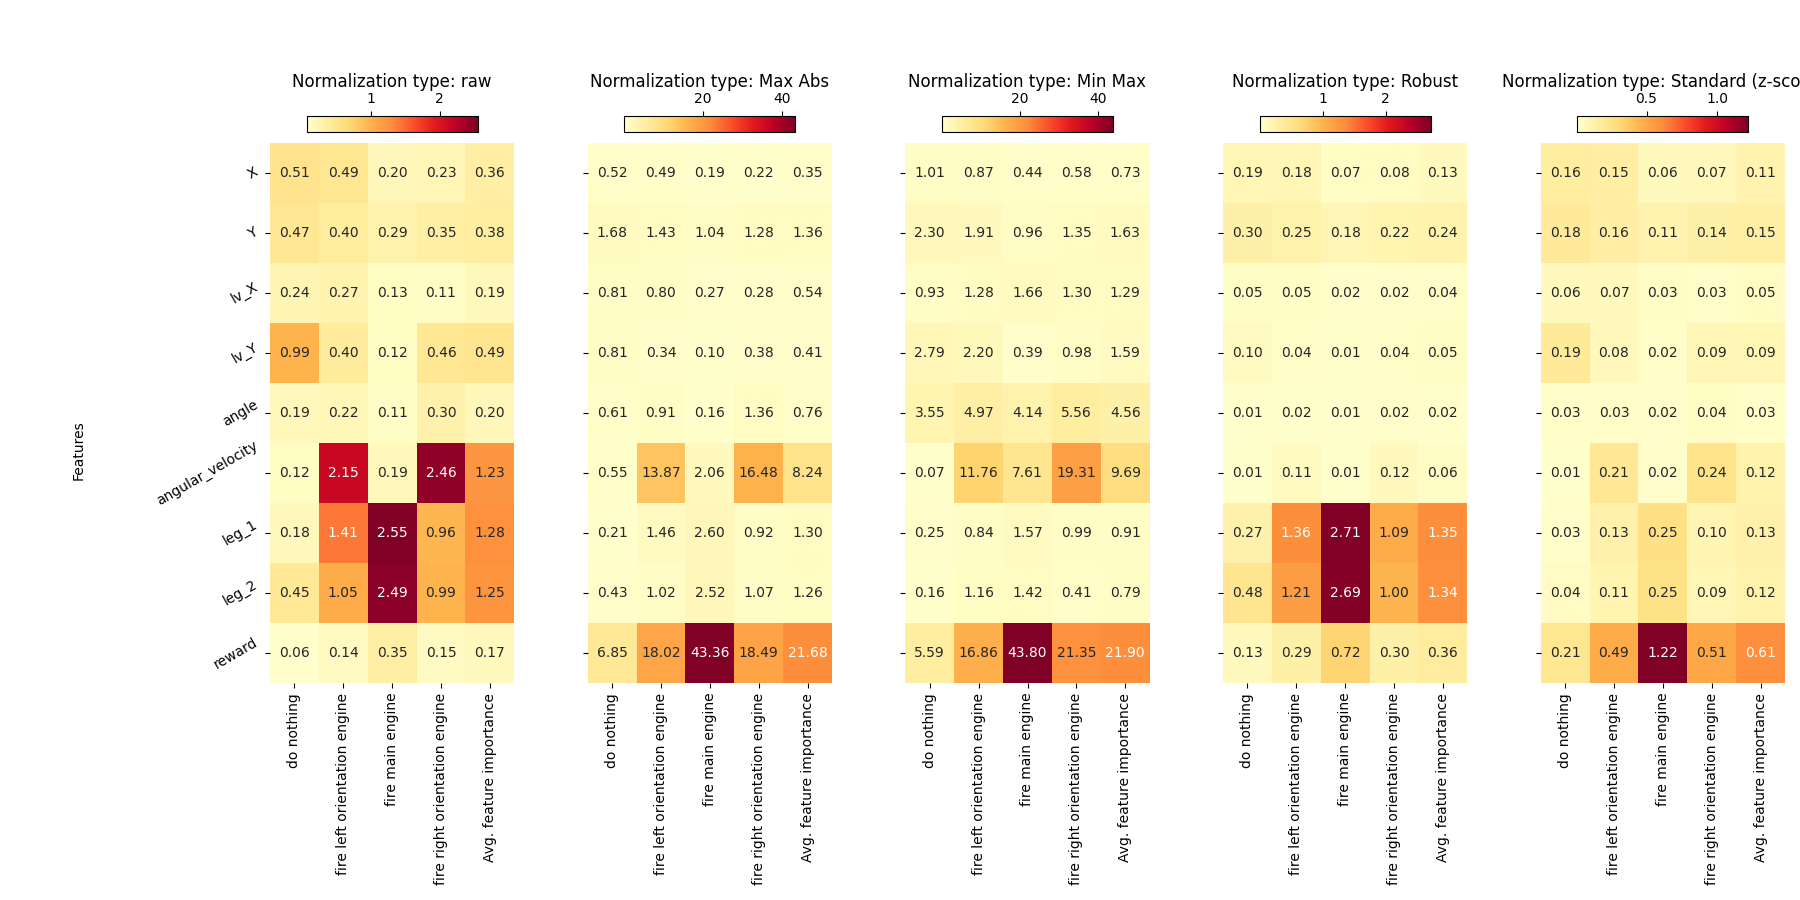
\includegraphics[width=1\linewidth]{images/data_exploration/rb_feature_importance_fig.png}
\caption{
Feature importance for the RB dataset using different normalization techniques on the training data.
}
\label{fig:rb_feature_importance}
\end{figure}

\begin{figure}[!b]
\centering
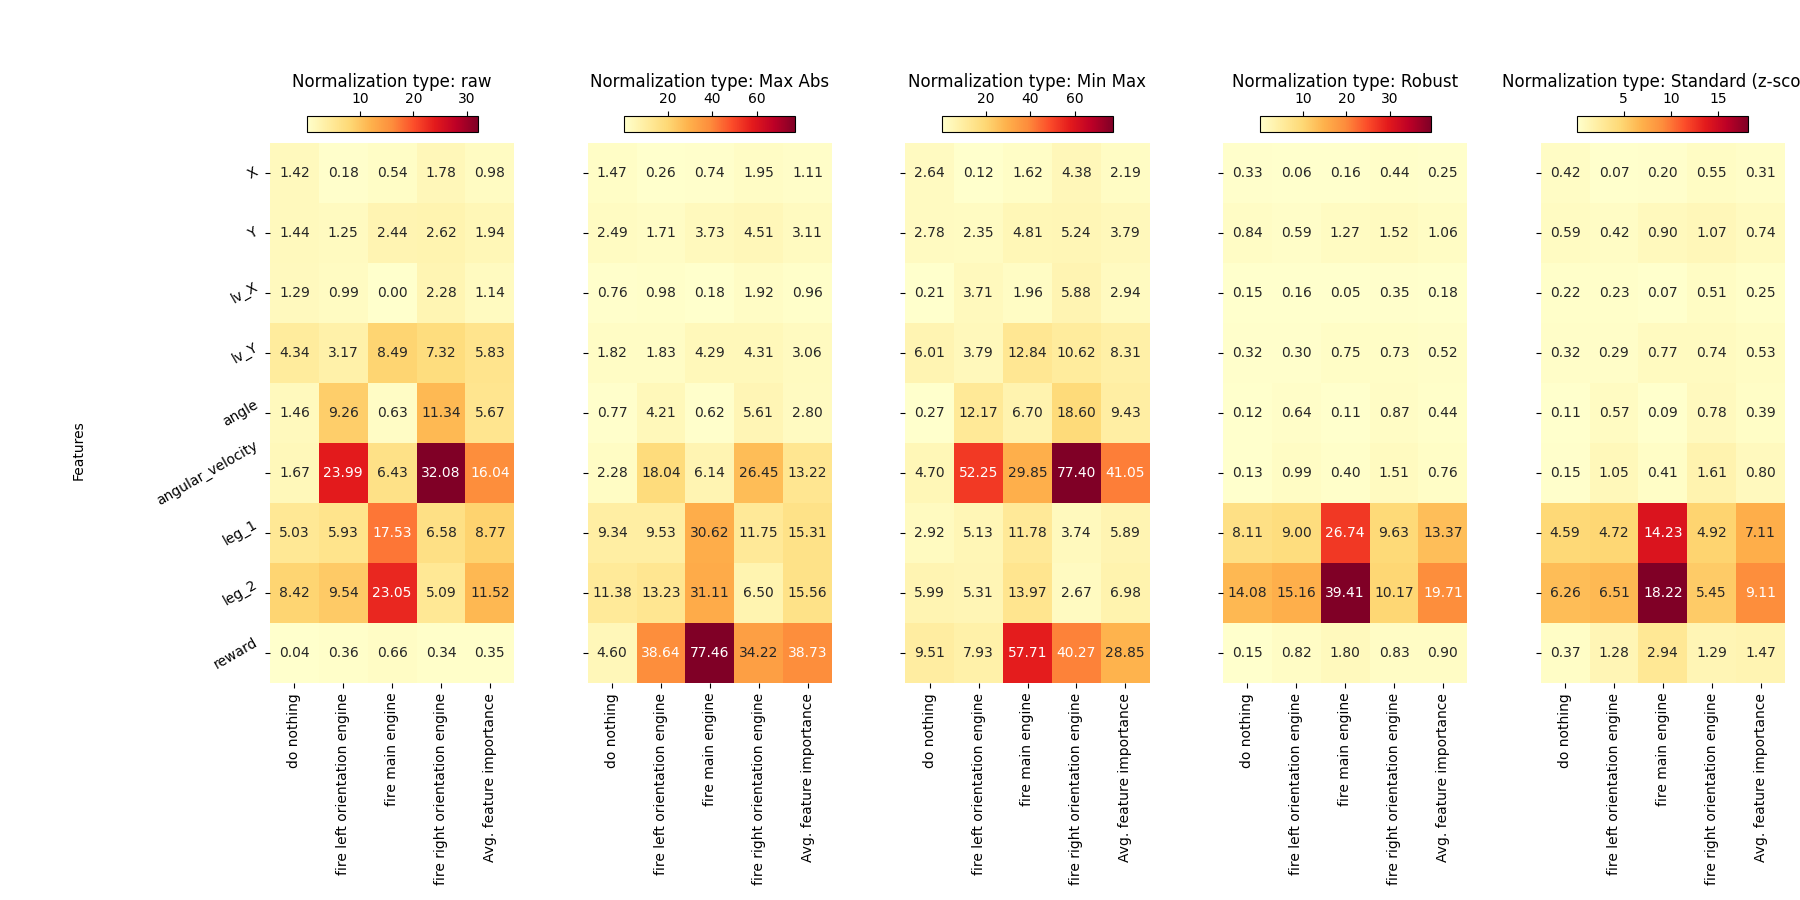
\includegraphics[width=1\linewidth]{images/data_exploration/fp_feature_importance_fig.png}
\caption{
Feature importance for the FP dataset using different normalization techniques on the training data.
}
\label{fig:fp_feature_importance}
\end{figure}

To understand which state dimensions provide the most information for action prediction, feature importance analysis was conducted on both the RB and FP datasets. For each dataset and normalization variant, a simple logistic regression classifier was trained. We chose logistic regression over tree-based methods because logistic regression classification is more similar to how FNNs handle states.

Feature importance is measured as the absolute value of the learned logistic regression coefficients. Larger values suggest stronger influence on action predictions. It is important to note that these values provide a general prediction on how informative the corresponding features are and not a definitive ranking of relevance \cite{hooker2019benchmark}. In FNNs, nonlinear transformations in hidden layers can change the importance of given dfeatures during training.




